% This LaTex template is for CPS 585 trem papers
%
%\documentclass[letterpaper]{article}
\documentclass[12pt, onecolumn]{article}
%
\usepackage[margin=1in]{geometry}
\usepackage[raggedright]{titlesec}
\usepackage[none]{hyphenat}
%
% include packages as needed, such as
\usepackage{amsmath}
%\usepackage{amsthm}
\usepackage{graphicx}
%\usepackage[ruled,vlined]{algorithm2e}
%\usepackage{array}
%\usepackage{multirow}
\usepackage{url}
\usepackage{enumerate}
\usepackage{listings}
\lstloadlanguages{Python}
%\usepackage{subfigure}
%etc.

%\setlength{\textwidth}{7.0in}
%\setlength{\textheight}{9.125in}
%\setlength{\columnsep}{0.375in}
%\setlength{\topmargin}{-0.8in}
%\setlength{\oddsidemargin}{-0.25in}
%\setlength{\evensidemargin}{-0.25in}
%\setlength{\parindent}{0.125in}
%\setlength{\parskip}{1mm}

\date{}

\titlespacing{\section}{0pt}{*2.0}{*2.0}
\titlespacing{\subsection}{0pt}{*1.8}{*1.8}

\renewcommand{\topfraction}{0.9}
\renewcommand{\textfraction}{0.1}

\begin{document}

% Change to your title
\title{\Large\textbf{Movie Recommendation System using Cosine Similarity}\normalsize}

%Chane authors, institutions and emails
\author {Amninder S Narota and Rajan Subramaniam \\
Department of Computer Science, Central Michigan University\\
Mount Pleasant, MI 48859\\
(narot1a, rajan1s)@cmich.edu
}
\maketitle 

\abstract{
In this paper, we compare commonly used distance measures in vector models, namely, cosine Angle Distance (CAD) queries in high dimensional data spaces. Using theoretical analysis and experimental results, we showed the retrieval results based on CAD when dimension is high. We have applied CAD for rating based similarity retrieval.

\section{Introduction} 


\subsection{Applications of Cosine Similarity}
Cosine similarity is an efficient method for calculating the similarity between the two independent object or vectors and it is used in the following applications:

\begin{enumerate}
	\item {\bf Text Mining: }In text mining the cosine similarity is used to find the similarity between the two documents by using the normalized score obtained from each document.
	
	\item {\bf Real-Time Traffic Classification: }Real - Time Traffic Classification covers the critical role of a network administrator to perform network, maintain the quality of service by performing efficient classification process using some statistical analysis process known as weighted cosine similarity.
	
	\item {\bf Semantic Similarity Calculation: }In semantic similarity calculation taxonomy based cosine similarity is used to find whether the two documents are similar or not.
	
	\item {\bf Direction of Motion Calculation in Routing Algorithms (EBGR): }Cosine similarity is one of the functional units used in Edge Node Based Routing which is used to find whether the peer nodes are in the direction of the destination node in a dynamic wireless network known as Vanet.
	
	\item {\bf Text Clustering: }Cosine similarity is used to find the similar word in a document there by reducing the unordered text documents into meaningful related clusters.
	
	\item{\bf Google's Page Rang Algorithm: }Cosine similarity is one of the statistical components used to formulate a web graph by calculating the page score obtained from each node from the search query pattern.

\end{enumerate}

%RELATED WORK
\section{Related Work}
Yehunda Koren\cite{Koren091the} in his article "\emph{The BellKor Solution to the Netflix Grand Prize}" explained about the algorithm Netflix is using for the movie recommendation system. The team of Netflix have more than 40 people hand-tagging TV shows and movies for them. These are typically freelancers who do this to supplement their income. All of their analysts are TV and movie buffs, and many have some experience working in the entertainment industry. They obviously have personal tastes, but their job as an analyst is to be objective.

Another important element in Netflix� personalization is awareness. They want members to be aware of how they are adapting to their tastes. Above all, the algorithm that was developed as part of Netflix million dollar prize are blends of a large number of different machine learning techniques. Two of the most notable aspects that emerged from the competition were using matrix factorisation and the so-called "temporal dynamics"\cite{Koren091the} to perform collaborative filtering; the full details can be found on the forum page (which has links to papers written by the winning team):
%METHODOLOGY
\section{Methodology}
In this project we are finding the similarities between the different movies by implementing cosine similarity concept on the user reviews obtained from different users. Angular similarity is a similarity metric obtained from the two movies which are considered as two documents by implementing cosine similarity between them. In general the cosine value will be between 0 and 1.If the cosine value of the two vectors are large then the inner product space between the vectors is large which means the two vectors have high degree of dissimilarity. If the cosine value is small then the inner product space between the vectors is small that denotes the two vectors are similar in nature.

Cosine Similarity\cite{dke} is a metric used to find the similarity between the two objects in terms of orientation. Here the two objects are considered as vectors in a user defined n dimensional space. The similarity is based only upon the orientation of the two different vectors and it does not consider the magnitude of the two vectors. The similarity level is generally based on the angle derived from the cosine similarity measure which denotes the cosine angular similarity between the two vectors. The two vectors are said to be similar if they have a smaller cosine angle. The smaller angle denotes the inner product space between the two vectors or objects are small which displays that the two vectors are similar. If the cosine angle is large there will be a large inner product space between the two vectors which denotes the two vectors are dissimilar to each other. 
\begin{align*}
\cos \theta &= \frac{A.B}{||A|| \text{ }||B|| }\\
&= \frac{\sum_{i=1}^{n} A_{i} \times B_{i}}{\sqrt{\sum_{i=1}^{n}(A_{i})^{2} \times \sum_{i=1}^{n}(B_{i})^{2}}}
\end{align*}

\begin{figure}[h!]
  \centering
    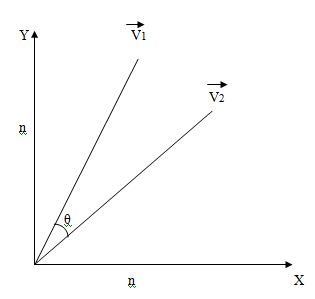
\includegraphics[natwidth=0.4\textwidth]{graph.JPG}
      \caption{Cosine angular similarity graph}
\end{figure}

\subsection{Term Definition}
Following are the term definitions we used in this project:
\begin{enumerate}
	\item{\bf Document: }Collection of item sets. Eg: Movie A, Movie B, Movie C etc.
	
	\item {\bf Item Sets: } Denotes the set of attributes related to the particular document. Eg: Movie ID, User rating, Date information.
	
	\item{\bf Term Frequency: } Measures the number of times the item set occur in a document.
	
	\item{\bf Normalized Term Frequency [NTF]: }To get the values (item sets) in range (normalized) we are dividing each value by the total number of values.
	
	\item {\bf Inverse Document Frequency [IDF]: }It is a potential score which denotes the weight of each item set in a document.
\end{enumerate}

\subsection{Formulas Used}
\label{sec: formulas}
\begin{enumerate}
	\item{\bf IDF[item set]}:
	\label{itm: idf_item}
		\begin{equation}
			\text{IDF[item set] }= 1 + \log_{e} ( \frac{\text{Total numbers of users}}{\text{Number of times the item set repeated}})
		\end{equation}
	
	\item{\bf Cosine Similarity: } Finds the similarity between the given item set with the stored item set in a document and generats the angular similarity between the two documents \emph{i.e} Movies.
	\label{itm: cosineFormula}
		\begin{equation}
		\label{eq: idf}
			\text{Cosine similarity (item-set, doc) } = \frac{\text{Dot product (item-set, Document)}}{||\text{item-set}||\text{ }\times ||\text{ Document}||}
		\end{equation}
\end{enumerate}

\subsection{Algorithm}
\begin{enumerate}[ {STEP }1{:}]
	\item Measuring the Term Frequency for each item set (user ratings) in a document (Movie). 
	\item Normalize the Term frequency to get into an appropriate value range.
	\item Generate Inverse Document Frequency (IDF) for each item-set (user ratings) in a document.
	\item Calculating the angular similarity between the two documents 
\end{enumerate}

\subsubsection{Calculation}
For explanation we created sample data for movies, say \emph{Movie A, Movie B} which are as follows:

\begin{enumerate}
	\item Normalized values for all the user ratings in Movie A are in Table \ref{tab: tabMovieA}
	
		{\bf Document 1: } Movie A\\
		{\bf Number of Users: }5\\
		{\bf Rating Limit: }5\\
		{\bf UR: }User Ratings\\
		{\bf NUR: }Normalized User Ratings		
		\begin{table}[ht]
		\label{tab: tabMovieA}
		
		\begin{center}
		\begin{tabular}{cccccc}
    		\hline
       			Number of Users	&	UR1	&	UR2	&	UR3	&	UR4	&	UR5\\
		\hline
    			UR				&	3	&	4	&	1	&	2	&	1\\
			NUR				&	0.6	&	0.8	&	0.2	&	0.4	&	0.2\\
    		\hline
		\end{tabular}
		\caption{Document 1; Movie A}
		\end{center}
		\label{tab:movieA}
		\end{table}
		
	\item Normalized values for all the user ratings in Movie B are in Table \ref{tab: tabMovieB}.
	
		{\bf Document 2: } Movie B\\
		{\bf Number of Users: }5\\
		{\bf Rating Limit: }5\\
		{\bf UR: }User Ratings\\
		{\bf NUR: }Normalized User Ratings	
		\begin{table}[ht]
		\label{tab: tabMovieB}
		\begin{center}
		\begin{tabular}{cccccc}
    		\hline
       			Number of Users	&	UR1	&	UR2	&	UR3	&	UR4	&	UR5\\
		\hline
    			UR				&	3	&	2.5	&	3	&	5	&	4\\
			NUR				&	0.6	&	0.5	&	0.6	&	1	&	0.8\\
    		\hline
		\end{tabular}
		\caption{Document 2; Movie B}
		\end{center}
		\label{tab:movieB}
		\end{table}
		
	\item Inverse Document Frequency [IDF] is calculated using \emph{Equation \ref{eq: idf}} of Section \ref{sec: formulas} Item \ref{itm: idf_item} and result is in \emph{Table \ref{tab: tabidf}}
	\begin{table}[ht]
	\label{tab: tabidf}
		\begin{center}
		\begin{tabular}{|c|c|c|}
    		\hline
       			Users	&	IDF Calculation					&	IDF\\
		\hline
    			U1		&	$1+\log_{e}(\frac{10}{3})$			&	2.2039\\
			U2		&	$1+\log_{e}(\frac{10}{2})$			&	2.6094\\
			U3		&	$1+\log_{e}(\frac{10}{2})$			&	2.6094\\
			U4		&	$1+\log_{e}(\frac{10}{1})$			&	3.3025\\
			U5		&	$1+\log_{e}(\frac{10}{2})$			&	2.6094\\
			U6		&	$1+\log_{e}(\frac{10}{3})$			&	2.2039\\
			U7		&	$1+\log_{e}(\frac{10}{3})$			&	3.3025\\
			U8		&	$1+\log_{e}(\frac{10}{3})$			&	2.2039\\
			U9		&	$1+\log_{e}(\frac{10}{1})$			&	3.3025\\
			U10		&	$1+\log_{e}(\frac{10}{2})$			&	2.6094\\
			
			
    		\hline
		\end{tabular}
		\caption{IDF Values}
		\end{center}
		\label{tab:movieB}
		\end{table}
	
	\item Normalized values for all the user ratings in Movie C are in Table \ref{tab: tabMovieC}.
	
	{\bf Given Document: } Movie C\\
		{\bf Number of Users: }2\\
		{\bf Rating Limit: }5\\
		{\bf UR: }User Ratings\\
		{\bf NUR: }Normalized User Ratings	
		\begin{table}[ht]
		\label{tab: tabMovieC}
		\begin{center}
		\begin{tabular}{ccc}
    		\hline
       			Number of Users	&	UR1	&	UR2	\\
		\hline
    			UR				&	2.5	&	1.5	\\
			NUR				&	0.5	&	0.3	\\
    		\hline
		\end{tabular}
		\caption{Document 2; Movie B}
		\end{center}
		\label{tab:movieB}
		\end{table}

	\item Creating (UR $\times$ IDF) matrix for the given document - Movie C and result is in Table \ref{tab: tabMovieC}
	
	\begin{table}[ht]
		\label{tab: tabMovieC}
		\begin{center}
		\begin{tabular}{ccc}
    		\hline
       			Number of Users	&	IDF	&	UR$\times$IDF	\\
		\hline
    			0.5				&	3.3025	&	1.6512	\\
			0.3				&	2.6094	&	0.7828	\\
    		\hline
		\end{tabular}
		\caption{(UR $\times$ IDF)}
		\end{center}
		\label{tab:URIDF}
		\end{table}
		
		
	\item Createing (UR $\times$ IDF) matrix by comparing Movie C with Movie A and Movie B. The values are in Table \ref{tab: movaVSmovb}
	
	\begin{table}[ht]
	\label{tab: movaVSmovb}
		\begin{center}
		\begin{tabular}{ccc}
    		\hline
       			Movie C	&	Movie A	&	Movie B	\\
		\hline
    			0.5				&	1.321	&	1.6512	\\
			0.3				&	0.5218	&	0	\\
    		\hline
		\end{tabular}
		\caption{(UR $\times$ IDF)}
		\end{center}
		\label{tab:URIDF}
		\end{table}
	
	\item Cosine Similarity between two movies can be calculated using the formula in  \emph{Equation \ref{eq: idf}} of Section \ref{sec: formulas} Item \ref{itm: cosineFormula}. Cosine Similarity between Movie C and Movie A is:
	
	\begin{align*}
		\text{Cosine Similarity(Movie C, Movie A) } &= \frac{(1.6512 \times 1.321)+(0.7828\times 0.5218)}{\sqrt{(1.6512^{2}+0.7828^{2})\times (1.321^{2}+0.5218^{2})}} \\
		&= 0.99 \\
		\\
		\text{Cosine Similarity(Movie C, Movie B) } &= \frac{(1.6512 \times 1.6512)+(0.7828\times 0)}{\sqrt{(1.6512^{2}+0.7828^{2})\times (1.6512^{2}+0)}} \\
		&= 0.90 \\
	\end{align*}
	
	The Cosine Similarity shows the cosine angle between two matrices. The cosine similarity between Movie C and Movie B is smaller when compared to cosine similarity between Movie C and Movie A. Hence with the small cosine value denotes that the inner product space between Movie C and Movie B is small thereby stating that Movie C is more similar to Movie B when compared to Movie A in terms of user ratings. 
\end{enumerate}

\subsection{Development}
For the development of this project our development environment was Python and to fine Cosine Similarity we used the following libraries:

\begin{enumerate}
	\item{\bf recsys: }python-recsys is build on top of Divisi2. It is used to calculate cosine similarity calculation
	\item{\bf Divisi2: }Divisi is particularly designed for working with knowledge in semantic networks.
	\item{\bf SciPy: } It is a computing environment and open source ecosystem of software for the Python programming language used by scientists, analysts and engineers doing scientific computing and technical computing.
	\item{\bf Numpy: }NumPy is the fundamental package for scientific computing with Python. It contains among other things:
		\begin{itemize}
			\item a powerful N-dimensional array object
			\item sophisticated (broadcasting) functions
			\item tools for integrating C/C++ and Fortran code
			\item useful linear algebra, Fourier transform, and random number capabilities
		\end{itemize}
\end{enumerate}

The contents of \emph{movie.dat} are stored in the variable \emph{movieNames} and \emph{ratings.dat} is stored in \emph{ratings}. Every movie name is allotted an unique ID and \emph{movie\_dict} is dictionary variable defined to map name to the id of the movie. The similarity matrix is stored in a form of dictionary mapping the movie with 10 top similar movies arranged in the defending order. This variable is then rendered in JSON file. \emph{svd} defined in method \emph{readDat()} as mentioned in Code snippet is used to store the data from the file and stored in the form of matrix.

The values of matrix is stored in \emph{svdlibc} by converting into sparse matrix. If a matrix A is stored in ordinary (dense) format, then the command $S = \text{sparse(A)}$ creates a copy of a matrix stored in sparse format. The rating of the movies are separated by \emph{::} in the following structure:
\begin{center}
	UserID :: MovieID :: Ratings :: TimeStamp
\end{center}
\begin{enumerate}
	\item {\bf UserID: } Every user who rating the movie is given an unique ID
	\item {\bf MovieID: } Every movie is given an unique ID
	\item {\bf Ratings: } This is the rating given by the user. The rating value is from 1 through 5.
	\item {\bf TimeStamp: }This is the date on which user rated the move title. It is the total seconds elapsed since 1\textsuperscript{st} of  January 1970.
\end{enumerate}


\begin{table}[ht]
		\begin{center}
		\begin{tabular}{c}
    		 \fbox{
			\parbox{\linewidth}{
				\lstinputlisting[label = samplecode, firstline=33,lastline=51]{movie.py}
			}
		}
		\end{tabular}
		\end{center}
		\label{tab:URIDF}
		\end{table}

The syntax to find the similarity between two documents is 
\begin{center}
	\emph{svd.similarity(item1, item2)} \\
	or \\
	\emph{svd.similar(item)}
\end{center}

Here \emph{svd} is the object which holds the computed vector matrix of similarity. To find all the similar values we used \emph{svd.similar(item)}. All the values are run through loops till it finds the end of movie file and finding all the similar values to the particular movie. All the similar movies are then stored in the form of list and mapped to the movie for which the value was to be found. Later this value is used to generate JSON file.\\ \\


 \fbox{
	\parbox{\linewidth}{
		\lstinputlisting[label = samplecode, firstline=52,lastline=59]{movie.py}
	}
}\\\\


 \fbox{
	\parbox{\linewidth}{
		\lstinputlisting[label = samplecode, firstline=60,lastline=64]{movie.py}
	}
}\\ \\


\emph{movie\_dict} is dictionary for mapping movie name to the movie id. It opens \emph{movie.dat} file and splits each line by "\emph{::}" and stores in the form if list. The movie id is at 0\textsuperscript{th} index and name is at 1\textsuperscript{st} index.\\\\


 \fbox{
	\parbox{\linewidth}{
		\lstinputlisting[label = samplecode, firstline=86,lastline=92]{movie.py}
	}
}\\ \\

\emph{dat\_to\_json(dict)} is method defined to create result in the form if JSON file from the dictionary provided as an argument. It opens "\emph{result.json}" file and writes \emph{movie\_name\_dict} value into the file.
\\\\

 \fbox{
	\parbox{\linewidth}{
		\lstinputlisting[label = samplecode, firstline=60,lastline=69]{movie.py}
	}
}\\ \\


This JSON file is used to render HTML web page linked to  {http://whispering-sands-8504.herokuapp.com}

\section{Experimental Results}

\section{Conclusion}


\bibliographystyle{plain}
\bibliography{myRefs} %change to your file name (with suffix .bib)


\end{document} 